\documentclass[12pt, a4paper, table]{article}
%\usepackage[utf8]{inputenc}
\usepackage[T1]{fontenc}
\usepackage[francais]{babel}
\usepackage{textcomp}
\usepackage{mathtools,amssymb,amsthm}
\usepackage[left = 2cm, top = 2cm, right = 2cm, bottom = 2.5 cm, headheight = 0pt]{geometry}
\usepackage{graphicx}
\usepackage{pgf, tikz}
	\usetikzlibrary{arrows,shapes,positioning}
\usepackage{centernot}
\usepackage{pgffor, ifthen}
\usepackage{lmodern}
\usepackage{colortbl}
\usepackage{array}
\usepackage{calc}
\usepackage{titlesec}
\usepackage{titletoc}
\usepackage{fancyhdr}
\usepackage{fancybox}
\usepackage{titling}
\usepackage{enumitem}
\usepackage{wrapfig}
\usepackage{caption}
\usepackage{tocloft}
\usepackage{epigraph}
\usepackage{lipsum}
\usepackage{ulem}
\usepackage{multirow}
\usepackage{hhline}
\usepackage{xcolor}
\usepackage{listings}
\usepackage{hyperref}
\definecolor{light-gray}{gray}{0.95}
\setcounter{tocdepth}{0}

\titleformat{\section}
  {\normalfont\sffamily\Large\bfseries}
  {\thesection.}{0.5em}{}

\titleformat{\subsection}
  {\normalfont\sffamily\large\bfseries}
  {\thesubsection}{0.5em}{}
\titleformat{\subsubsection}
  {\normalfont\sffamily\normalsize\bfseries}
  {}{0.5em}{}


\definecolor{pblue}{rgb}{0.13,0.13,1}
\definecolor{pgreen}{rgb}{0,0.5,0}
\definecolor{pred}{rgb}{0.9,0,0}
\definecolor{pgrey}{rgb}{0.46,0.45,0.48}


\lstset{language=Java,
 basicstyle=\footnotesize\tt,
  showspaces=false,
  showtabs=false,
  breaklines=true,
  showstringspaces=false,
  breakatwhitespace=true,
  commentstyle=\color{pgreen},
  keywordstyle=\color{pblue},
  stringstyle=\color{pred},
  moredelim=[il][\textcolor{pgrey}]{$$},
  moredelim=[is][\textcolor{pgrey}]{\%\%}{\%\%},
    numbers=left,
    numberstyle=\color{pgrey}, % the style that is used for the line-numbers
  rulecolor=\color{black}
}

\pagestyle{fancy}

\setlength{\headheight}{15pt} 

\renewcommand{\headrulewidth}{1pt}
\fancyhead[C]{} 
\fancyhead[L]{\textsf{Groupe 14 \\ Antoine Duchêne - Justin Michaux}}
\fancyhead[R]{\textsf{LSINF1103 \\ Introduction à l'algorithmique}}

\renewcommand{\footrulewidth}{1pt}
\fancyfoot[C]{}
\fancyfoot[R]{\textbf{\textsf{\thepage}}}
\fancyfoot[L]{\textbf{\textsf{\today}}}

\begin{document}


\begin{Large} \begin{center}
\noindent \rule{15cm}{.9pt} 
\vspace{-0.33cm}
	\textsf{Mini-projet 1 - Manipulation d'expressions arithmétiques}\\
	\rule{15cm}{.9pt} 
\end{center} \end{Large} 

\section{Diagramme des classes}
\begin{center}
\vspace{1cm}
	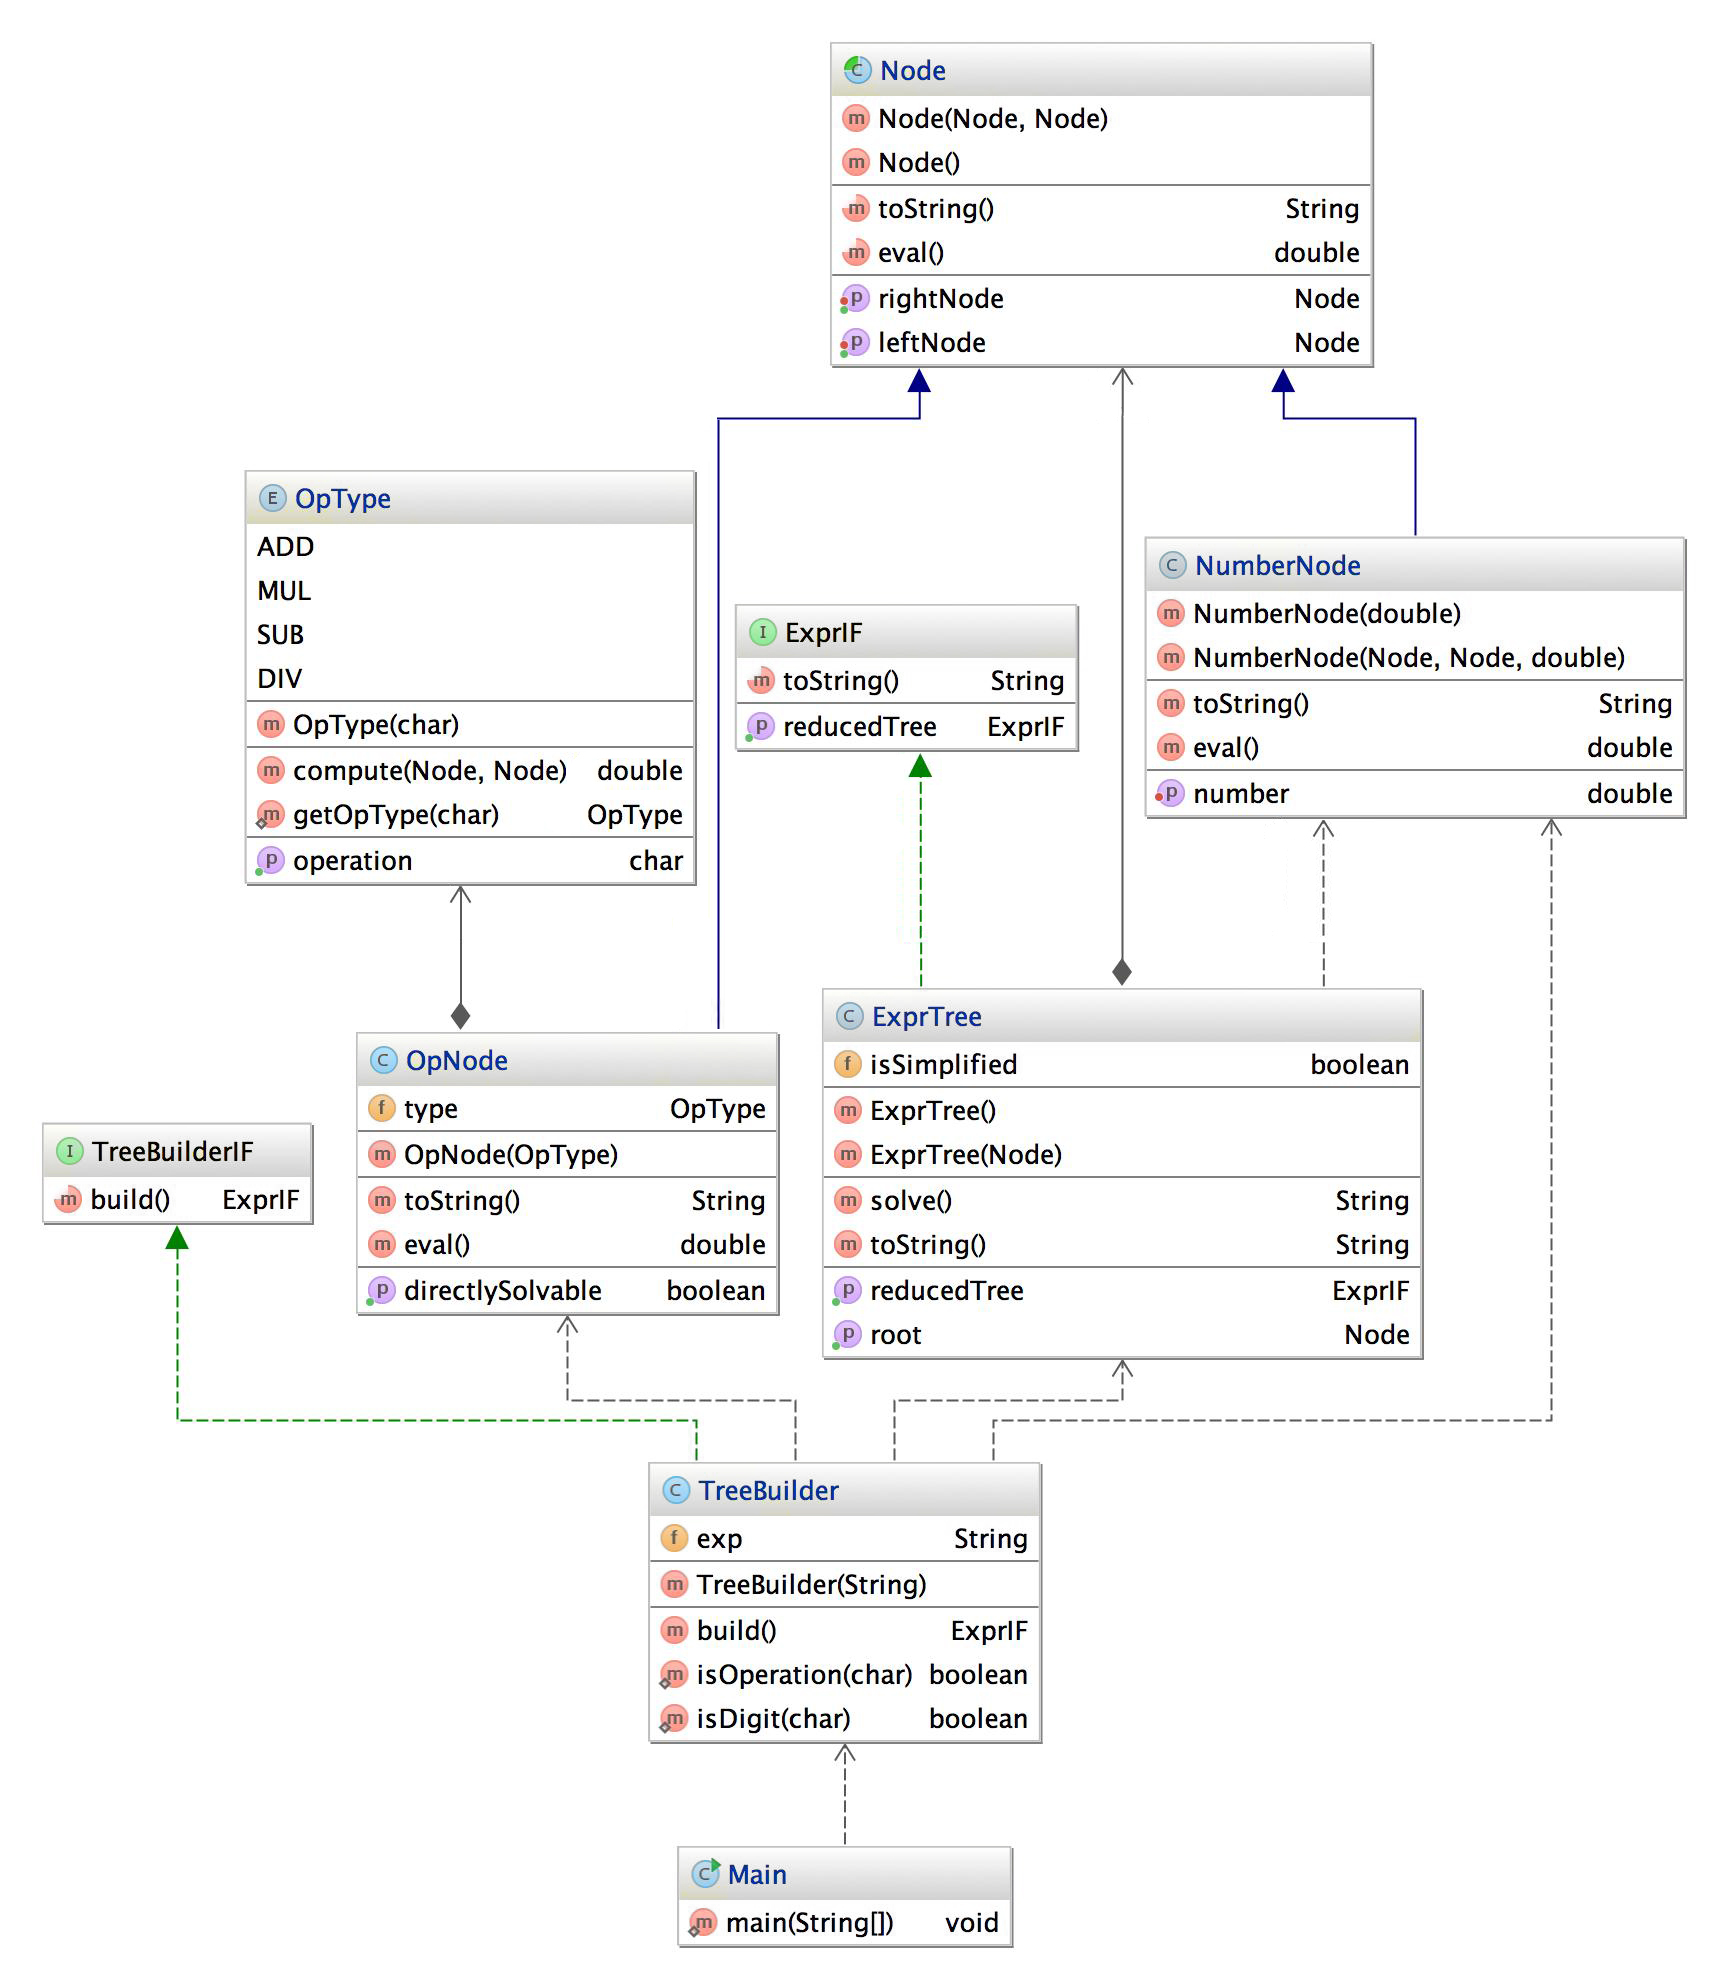
\includegraphics[width = 17cm]{diagramme}
\end{center}

\newpage

\fontfamily{phv}\selectfont
\section{Choix d'implémentation}
Afin d'implémenter l'arbre syntaxique abstrait, nous avons utilisé une structure chainée. Ce type d'implémentation a été préféré à un tableau dynamique car la complexité spatial avec un tableau est de $\mathbf{\Theta (2^{n})}$ alors qu'avec une structure chainée la complexité spacial est de $\mathbf{\Theta (n)}$.
\medskip

De plus, une structure chainée était un choix obligatoire vu la contrainte d'utiliser des méthodes récursives.
\vspace{-6pt}
\section{Complexité des différentes méthodes}
\noindent Soit n, le nombre d'opérations et de nombres : n représente donc la taille du problème à résoudre.
\vspace{-6pt}
\subsection{TreeBuilderIF.build()}
\noindent Complexité temporelle en $\mathbf{\Theta (n)}$ car :

\begin{enumerate}
	\item L'expression sera toujours parcourue entièrement 1 fois, à l'aide d'une boucle.
	\item La boucle principale ne contient que des opérations de complexité $\mathbf{\Theta (1)}$.
\end{enumerate}

\noindent On en déduit donc que le temps d'exécution augmentera de façon linéaire par rapport à la taille du problème.

\subsection{ExprIF.getReducedTree()}
\noindent Complexité temporelle en $\mathbf{\mathcal{O}(}\mathbf{log (n))}$ car :
\begin{enumerate}
	\item Complexité temporelle en $\mathbf{\mathcal{O}(h)}$, où h est la hauteur de l’arbre
	\item L'arbre est équilibré donc h $\in$ $\mathbf{\Theta(\mathbf{log}_{2} (n))}$
\end{enumerate}
Donc, 
\begin{itemize}
	\item Meilleur cas : $\mathbf{\Theta (1)}$ (on tombe sur la racine)
	\item Pire cas : $\mathbf{\Theta(}\mathbf{log (n))}$
	\item En général : $\mathbf{\mathcal{O}(}\mathbf{log (n))}$
\end{itemize}



\subsection{ExprIF.toString()}
\noindent Complexité temporelle en $\mathbf{\mathcal{O}(n)}$ car on passe, dans le pire des cas, 3x par chaque noeud de l'arbre (parcours d'Euler). On a donc une complexité en  $\mathbf{\mathcal{O}(3n)}$. On peut "simplifier" le 3 car il s'agit d'une constante. On obtient donc $\mathbf{\mathcal{O}(n)}$  

\begin{itemize}
	\item Meilleur cas : $\mathbf{\Theta (1)}$ (L'arbre est entièrement simplifié)
	\item Pire cas : $\mathbf{\Theta(n)}$
	\item En général : $\mathbf{\mathcal{O}(n)}$
\end{itemize}


\section{Difficultés rencontrées}
\begin{itemize}
	\item Quelques difficultés à implémenter une méthode récursive
	\item Choix d'implémentations
\end{itemize}



\newpage
\section*{Annexe}

\subsection*{TreeBuilder}

\begin{lstlisting}[language=Java]
public ExprIF build() {
    Stack<Node> stack = new Stack<Node>();
    for (int i = 0; i < exp.length(); i++) {
        char currentChar = exp.charAt(i);
        if (isDigit(currentChar)) {
            StringBuilder number = new StringBuilder();
            while (i < exp.length() && isDigit(exp.charAt(i))) {   //Tant que le nombre n'est pas fini
                number.append(exp.charAt(i));
                i++;
            }
            Node Node = new NumberNode(Double.parseDouble(number.toString()));
            stack.push(Node);

        } else if (isOperation(currentChar)) {

            Node Node = new OpNode(OpType.getOpType(currentChar));
            stack.push(Node);

        } else if (currentChar == ')') {
            Node rightNode = stack.pop();
            Node root = stack.pop();
            Node leftNode = stack.pop();
            root.setLeftNode(leftNode);
            root.setRightNode(rightNode);
            stack.push(root);
        }

    }
    return new ExprTree(stack.pop()); // Retourne la racine de l'AST
}\end{lstlisting}
\medskip
\subsection*{ExprIF}
\begin{lstlisting}
public String toString() {
    String str = null;
    if (root.getLeftNode() == null && root.getRightNode() == null) {
        return root.toString();
    } else if (root.getLeftNode() != null && root.getRightNode() != null) {
        ExprTree LeftTree = new ExprTree(root.getLeftNode());
        ExprTree RightTree = new ExprTree(root.getRightNode());
        str = "(" + LeftTree.toString() + root.toString() + RightTree.toString() + ")";
    }
    return str;
}
\end{lstlisting}
\newpage
\begin{lstlisting}
public ExprIF getReducedTree() {

    if (getRoot().getLeftNode() != null && getRoot().getRightNode() != null) {
        ExprTree subLeft = new ExprTree(root.getLeftNode());
        ExprTree subRight = new ExprTree(root.getRightNode());
        ExprTree eL = (ExprTree) subLeft.getReducedTree(); // Appel récursif
        ExprTree eR = (ExprTree) subRight.getReducedTree(); // Appel récursif

        if (getRoot() instanceof OpNode) {

            if (((OpNode) getRoot()).isDirectlySolvable() && (!eL.isSimplified || !eR.isSimplified)) {
                root = new NumberNode(root.eval());
                isSimplified = true;
                return this;
            }
        }

        if (eL.isSimplified) {
            this.getRoot().setLeftNode(eL.getRoot());
            return new ExprTree(this.getRoot());
        }

        if (eR.isSimplified) {
            this.getRoot().setRightNode(eR.getRoot());
            return new ExprTree(this.getRoot());
        }


    }
    return this;
}
\end{lstlisting}








\end{document}